\documentclass[12pt,a4paper]{article}
\usepackage[useregional]{datetime2}
\usepackage[pdf]{graphviz}
\usepackage{hyperref}
\usepackage[backend=biber,style=numeric,sorting=none]{biblatex}
\usepackage[utf8]{inputenc}
\usepackage[final]{listings}
\usepackage{color}
\usepackage{amsmath}
\usepackage{xparse}
\usepackage[T1]{fontenc}
\usepackage{enumerate}
\usepackage{CJKutf8}
\usepackage{pifont}
\usepackage{tikz}
\usepackage{graphicx}
\usepackage{subcaption}
\usepackage{wrapfig}
\usepackage{indentfirst}
\usetikzlibrary{positioning, fit}
\graphicspath{{./images/}}
\usepackage{geometry}
\geometry{margin=2cm}
\setlength{\parindent}{2em}

\definecolor{mygreen}{rgb}{0,0.6,0}
\definecolor{mygray}{rgb}{0.5,0.5,0.5}
\definecolor{mymauve}{rgb}{0.58,0,0.82}
\addbibresource{mergedBib.bib}

% Link conf.
\hypersetup{
    citecolor=blue,
    colorlinks=true,
    linkcolor=blue,
    filecolor=magenta,      
    urlcolor=cyan,
    pdfpagemode=UseNone
}
\urlstyle{same}

% Code conf.
\lstset{ 
  backgroundcolor=\color{white},   % choose the background color; you must add \usepackage{color} or \usepackage{xcolor}; should come as last argument
  basicstyle=\ttfamily\footnotesize,% the size of the fonts that are used for the code
  breakatwhitespace=false,         % sets if automatic breaks should only happen at whitespace
  breaklines=true,                 % sets automatic line breaking
  captionpos=b,                    % sets the caption-position to bottom
  commentstyle=\color{mygreen},    % comment style
  deletekeywords={...},            % if you want to delete keywords from the given language
  escapeinside={\%*}{*)},          % if you want to add LaTeX within your code
  extendedchars=true,              % lets you use non-ASCII characters; for 8-bits encodings only, does not work with UTF-8
  frame=single,	                   % adds a frame around the code
  keepspaces=true,                 % keeps spaces in text, useful for keeping indentation of code (possibly needs columns=flexible)
  keywordstyle=\color{red},        % keyword style
  morekeywords={*,...},            % if you want to add more keywords to the set
  numbers=left,                    % where to put the line-numbers; possible values are (none, left, right)
  numbersep=5pt,                   % how far the line-numbers are from the code
  numberstyle=\tiny\color{mygray}, % the style that is used for the line-numbers
  rulecolor=\color{black},         % if not set, the frame-color may be changed on line-breaks within not-black text (e.g. comments (green here))
  showspaces=false,                % show spaces everywhere adding particular underscores; it overrides 'showstringspaces'
  showstringspaces=false,          % underline spaces within strings only
  showtabs=false,                  % show tabs within strings adding particular underscores
  stepnumber=1,                    % the step between two line-numbers. If it's 1, each line will be numbered
  stringstyle=\color{mymauve},     % string literal style
  tabsize=4,	                     % sets default tabsize to ˋ spaces
  title=\lstname,                  % show the filename of files included with \lstinputlisting; also try caption instead of title
  extendedchars=true,
}


\title{{The Container Security in Healthcare Data Exchange System}}
\author{Chih-Hsuan Yang\\
National Sun-Yet-San University, Taiwan \\
Bachelor's degree graduation project \\
Advisor: Chun-I Fan
}

\date{\today}



\begin{document}
% Cover page
% \maketitle
% \newpage
% \tableofcontents
% \newpage
% ================ Abstract ================
\section{Abstract}
Recently, many companies use containers to run their microservices since containers could
make their hardware resources be used efficiently. And the newest healthcare data exchange
standard FHIR (Fast Healthcare Interoperability Resources) \cite{FHIR_home} has been implemented
in a container by IBM, Microsoft, and firebase. The deployment of FHIR in a container is a
trend in the digital world \cite{Infrastructures}. However, if a hacker gets privilege
escalation of containers, then such attacks would influence the host or the other containers.
Therefore, this research would analyze, implement, and protect the container escalation
in healthcare data exchange system. The container escalation would be inspired in a container
and influence the host or the other containers. The healthcare data exchanging system will
take FHIR to simulate the real-world threat and purpose soliciting a secure solution to
protect patient's privacy.

% ================ Motivation ================

\section{Introduction and Motivation}
The Container is a virtualization technique to package applications and dependencies to run in
an isolated environment. Containers are faster to start-up, lighter in memory/storage usage
at run time, and easier to deploy than virtual machines. This is because that the container
shares the kernel with the host OS and other containers and deploys by a configure file
\cite{Offloading}. In this way, the information service based on a container platform increases
the resource efficiency of the system \cite{Comparison}.
First, we often used to run a docker container to host our services, for example: the
servers and some services in the information security club at NSYSU(National Sun Yat-sen University).
However, there are some threats to the container technique, such as "Dirty CoW" \cite{Dirty_CoW}
and "escape vulnerabilities".\\

Dirty CoW is a vulnerability in the Linux kernel. It is a local privilege escalation bug
that exploits a race condition in the implementation of the copy-on-write mechanism in the
kernel's memory-management subsystem \cite{Dirty_CoW_wiki}. It was found by Phil Oester. We
were 16, the first year we touched the docker container. We tried to use the Dirty CoW
vulnerability to take the root privilege of my Android phone.\\

Escape vulnerability is a subcategory of sandbox security. At first, security researchers often
need a sandbox to help them analyze malware, which prevents the malware influence researchers'
host OS. Nowadays, the sandbox not only is used in analyzing, but also used to execute a
normal application for an isolated environment. However, if the application could modify the
outside resources without the kernel permission, it will be unable to achieve the purpose of
isolation. That might cause the information leakage or the kernel being hacked.\\

Hence, there is a big problem: "How to make sure my services isolated and secure?"
We are leading the information security club at NSYSU. We should maintain all
the services working perfectly. Moreover, we are an information security club. Therefore,
the security and performance issue is the top-priority requirement.\\

Second, to present the container security, we would take the medical system as an example.
Our medical system is the most famous one internationally. When facing COVID-19
in Taiwan, we have not had any local COVID-19 case in more than 250 days \cite{COVID19_CNN}.
Medical workers usually needs to renew the EHR (Electronic Health Records)
system frequently. To protect the privacy of patients and producing a high-performance
system to exchange the EHR, an easy-deployment, effective-execution, and secure system is
required. It also is the major goal of this project.

% ================ Related works ================

\section{Related Works}
This section will focus on (\RN{1}) \hyperlink{preliminaries}{preliminaries} (\RN{2}) \hyperlink{security}{containter security}, and (\RN{3})
\hyperlink{heigh_performance}{high-performance server}.

\subsection{Preliminaries}
\hypertarget{preliminaries}{}
\subsubsection{FHIR}
FHIR is a standard for healthcare data exchange. The FHIR standard will be used
in Taiwan in the near future \cite{MOHW_FHIR}. FHIR will be used to provide PHR
(Personal Healthcare Records) in Taiwan. Therefore, we choose the most popular standard
"FHIR" for the target.

\subsubsection{Linux Kernel Features}
First, there are four basic features for the abstract containerization services in the
Linux environment.
The four basic features are: (\RN{1}) namespace, (\RN{2}) cgroups, (\RN{3}) capabilities,
and (\RN{4}) seccomp.

\paragraph{Namespaces}
The Linux kernel provides the namespaces to perform the job of isolation and virtualization
of system resources for a collection of processes \cite{Road_Ahead}.
User namespaces can be nested; that is, each user namespace—except the initial ("root")
namespace—has a parent user namespace and can have zero or more child user namespaces
\cite{user_namespaces}.

\begin{wrapfigure}[13]{r}{6cm}
  \centering
  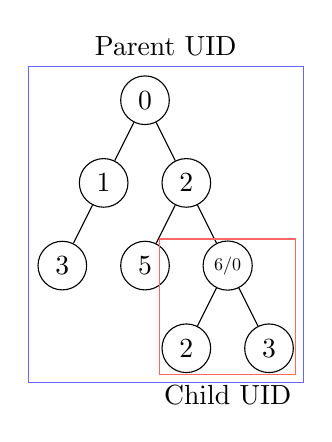
\begin{tikzpicture}[
      roundnode/.style={circle, draw=green!60, fill=green!5, very thick, minimum size=7mm},
      squarednode/.style={rectangle, draw=red!60, fill=red!5, very thick, minimum size=5mm},
      scale=0.7
    ]
    %Nodes
    \node[circle,draw](z){0}
    child{node[circle,draw]{1} child{node[circle,draw] (p_4){3}} child[missing]}
    child{node[circle,draw]{2} child{node[circle,draw] {5}}
        child{node[circle,draw, scale=0.65](n_1){6/0} child{node[circle,draw](n_2){2}} child{node[circle,draw](n_3){3}} } };
    \node[draw=blue!60, fit=(z)(n_2)(n_3)(p_4), label={Parent UID}] {};
    \node[draw=red!60, fit=(n_1)(n_2)(n_3), label=below:{Child UID}, scale=0.9] {};

  \end{tikzpicture}
  \caption[]{The nested user namespaces}
  \label{Nested}

\end{wrapfigure}
The nested namespace is shown in Figure \ref*{Nested}.

\paragraph{Cgroups}
This feature can limit, account for, and isolate the hardware resource usage of a
collection of processes \cite{cgroup_wiki}.
The container could use this feature to set the maximum/minimum usage of hardware
resources, which could guarantee processes' resources using reasonability.

\paragraph{Capabilities}
This feature divides the privileges traditionally associated with superuser into
distinct units. To perform permission checks, traditional UNIX
implementations distinguish two categories of processes: privileged and unprivileged.
Privileged processes would bypass all kernel permission checks, while unprivileged
processes are subject to full permission checking based on the processes' credentials
\cite{capabilities}.

Take the ping command as an example. The ping needs to generate and receive ICMP packets
and usually is generated by "raw sockets" – a feature limited to root only
(CAP\_NET\_RAW). Because it could also be abused to sniff and disrupt other traffic
on the systems. Moreover, we can set the capability to the file to get accessibility
to execute the file.
Therefore, when we set the CAP\_NET\_RAW capability to the /bin/ping, we could execute
the ping command as the users.

\paragraph{Seccomp}
The seccomp feature is that only some specified process could call some specified
system calls. We could set a policy while some file is loaded, and we often use
this system call to enforce the whitelisting or blacklisting policy.

Second, there are three terminologies of computer science related to container
security in the Linux kernel, which are (\RN{5}) mmap, (\RN{6}) Copy on write,
and (\RN{7}) Race condition.

\paragraph{`mmap`}
This is a system call of mapping files or devices into memory, which creates a
new mapping in the virtual address space of the caller process such that
the process could operate the instance of a file in memory directly.
And some libraries are also mapped into the virtual address space to share and handle
the function call. Therefore, the processes could take the same view of libraries in
its memory space.

\paragraph{Copy on Write}
This mechanism purposes that a resource is duplicated but not modified, and it is not
necessary to create a new entry. Therefore, the kernel can make callers share
the same memory resources. The mmap is a system call that could inspire this
mechanism in the above paragraph. When some processes request the same memory resource,
the kernel supplies the same memory page to the callers.

\paragraph{Race Condition}
This means that processes or threads are racing the same mutable resource. For example:
There is an accessible and mutable shared memory which is isnitialized as zero. And
two threads or processes are sharing that page. Consider that one of the tasks is assigning
the page full of character 'A'. In the meanwhile, the schedular context switches to
the other task, which assigns that page full of 'B'. Then the schedular context switches
again to the first task. There is a problem now. What is the page for the first
task looked like? It does not meet the expectation for the first task.
This is race condition.

Finally, there are two I/O Linux system calls that would be considered to enhance
the I/O performance, which are the (\RN{8}) epoll and (\RN{9}) io\_uring.

\paragraph{`epoll`}
The `epoll` system call is a scalable I/O event notification facility. Its function
is to monitor multiple file descriptors to see whether I/O is possibly on any of
them, which uses RB-tree to search the monitored file descriptors.

\paragraph{`io\_uring`}
The io\_uring system call is a new feature in the Linux kernel 5.1, which is also an
asynchronous I/O API, supplying larger throughput and lower latency. This system call
has three key elements: Submission Queue (SQ), Completion Queue (CQ), and Submission Queue
Entries (SQE).

When we operate the io\_ring, we should use the mmap to share the memory page from
the returned file descriptor by the io\_setup. After the page is mmaped, we could share
the three key elements with the Linux kernel. The Linux kernel will pick up our submission
from the SQE and polling in the kernel thread. That is, it is useless for a system call
to tell the kernel that we want to have an asynchronous I/O.

After the kernel finishes the I/O operation, the kernel will put the index of the finished
file descriptor to the completion queue. The user could traverse over the CQ to pick up
the finished file descriptors, which also reduced a system call to tell the kernel that
we picked it up.

Therefore, we do not require any system call on submission and completion in optimal cases.

\subsection{Container Security}
\hypertarget{security}{}
\subsubsection{The Dirty Copy on Write}
Delwar Alam, et al. \cite{Study_Dirty_Cow} showed the race condition and the mechanism of
"Copy on Write". "Copy on Write" is a resource-management technique used in
computer programming to efficiently implement a "duplicate" or "copy" operation
on modifiable resources \cite{CoW_wiki}. It is often inspired when `fork` or `mmap`.

\subsubsection{Dirty CoW Demo Code}
Let's analyze the proof of concept (PoC) of the dirty CoW \cite{Dirty_CoW} vulnerability.
The key of inspiring this vulnerability is the mmaped memory space, which is mapped with
the PROT\_READ flag. The PROT\_READ flag declares that the page is read-only.
\lstinputlisting[language=C, linerange={87-89, 101-101}, firstnumber=87]{src/dirtyc0w.c}

It creates two threads, which would have a race condition of the mmaped memory space,
\hyperlink{madvise}{madviseThread} and \hyperlink{procself}{procselfmemThread}.

\hypertarget{threads_main}{threads in main}
\lstinputlisting[language=C, linerange={106-107}, firstnumber=106]{src/dirtyc0w.c}

In one thread, issuing a system call `madvise`, would make the user thread gain the root
privilege to operate the protected page temporarily. And the flag MADV\_DONTNEED would
tell the kernel: "Do not expect to access it in the near future \cite{Madvise}." Moreover,
this flag might not lead to immediate freeing of pages in the range. The kernel is free
to delay free the pages until an appropriate moment \cite{Madvise}.

\hypertarget{madvise}{madviseThread}
\lstinputlisting[language=C, linerange={33-39,45-48}, firstnumber=33]{src/dirtyc0w.c}

In another thread, open its memory resource file. This file is a special file, which allows
the process to read its memory by itself.\\

Then, we move the printer of file descriptor of the memory resource file to the mmaped
space. And we try to write it. But the mmaped space is read-only. We expected that the
kernel would create a copy of this space and write the copy \cite{root_exploit}.\\
\hypertarget{procself}{procselfmemThread}
\lstinputlisting[language=C, linerange={50-53,61-63,67-71}, firstnumber=50]{src/dirtyc0w.c}

However, there is a problem! There is another thread that is racing this page with root
privilege. If the schedular context switches the madviseThread to procselfmemThread while
the adviseThread is calling the "madvise" system call, it would cause the
procselfmemThread to gain the root privilege from madviseThread to control the mmaped file.

\subsubsection{Container Security: Issues, Challenges, and Road Ahead}
Sari Sultan et al. \cite{Road_Ahead} have derived four generalized container security issues:
(\RN{1}) protecting a container from applications inside it, (\RN{2}) inter-container
protection, (\RN{3}) protecting the host from containers, and (\RN{4}) protecting containers
from a malicious or semi-honest host \cite{Road_Ahead}.

The (\RN{1}), (\RN{3}), and (\RN{3}) issues could implement the protection by the software
based solutions.

For the (\RN{1}) issue, Sari Sultan et al. \cite{Road_Ahead} recommends that
we could use the different capabilities and the LSM (Linux secure module). Take
CVE-2017-5123 \cite{CVE-2017-5123} as an example. The vulnerability here is the third argument of
`waitpid` system call which didn't ensure that the user-specified pointer points to user space
and not kernel space since unprivileged users shouldn’t be able to write arbitrarily
to kernel memory.

The solution of CVE-2017-5123 without updating the Linux kernel is to insert an
LSM to the kernel, which monitors the runtime behaviors of system calls. If any process
uses the waitpid() with a pointer point to the kernel as the third argument, the LSM should
block the operation and raise a signal to the user.

For the (\RN{2}) issue \cite{Road_Ahead} recommends that we could use the
LSM, namespaces, and cgroups to limit the container. Take CVE-2016-8655 \cite{CVE-2016-8655,Measurement}
as an example. This vulnerability is a bug in net/packet/af\_packet.c. We often use the
CAP\_NET\_RAW namespace in the container to make unprivileged user be able to use some privileged
net-util commands. The bug is that there exists a race condition probability to race the unauthorized
data inside packet\_set\_ring() and packet\_setsockopt() \cite{CVE-2016-8655-lwn} such that
there is a chance to modify the socket version to TPACKET\_$V_1$ before the packet\_set\_ring
function. However, it would be `kfree` the timer in the TPACKET\_$V_1$. We can take the timer,
which is used after free, to control the SLAB adopter to write the st\_uid by itself
\cite{AF_PACKET}.

For the (\RN{3}) issue, we take the Dirty CoW vulnerability as an example, which is exploitation
from the Linux kernel. The vulnerability could change the victim container to be a privileged
container. Therefore, we should protect the host from the container, which belongs to type
(\RN{3}) threat.

\subsection{High-Performance Server}
\hypertarget{heigh_performance}{}
This section will study some I/O performance and caching issues because the healthcare
data exchange system demands the stringent specification of the response time.
The I/O is the most often one causing the bottleneck in the low latency required system.
To support a high-performance system, we can design a module to control the throughput
intelligently, and use the cache-friendly architecture to minimize the latency.

\subsubsection{PINE: Optimizing Performance Isolation in Container Environments}
Youhuizi Li et al. \cite{Optimizing} introduced a high throughput and low latency module to control
the I/O streams. It implements a module to accord calculated optimization parameters,
and checks if the process throughput is satisfied or the 99.9\% throughput is satisfied.

If the throughput reached the bottleneck, then the model would extend the
bandwidth by the cgroup. The latency evaluation is more difficult than throughput
evaluation. Youhuizi Li et al. \cite{Optimizing} evaluated if the latencies of 99.9\% of the
data are all within three standard deviations of the acceptable latency. If not,
the module will raise the priority of the I/O queue.

\subsubsection{`epoll` vs. `io\_uring` Performance Comparison}
\begin{wrapfigure}[8]{r}{.45\textwidth}
  % \centering
  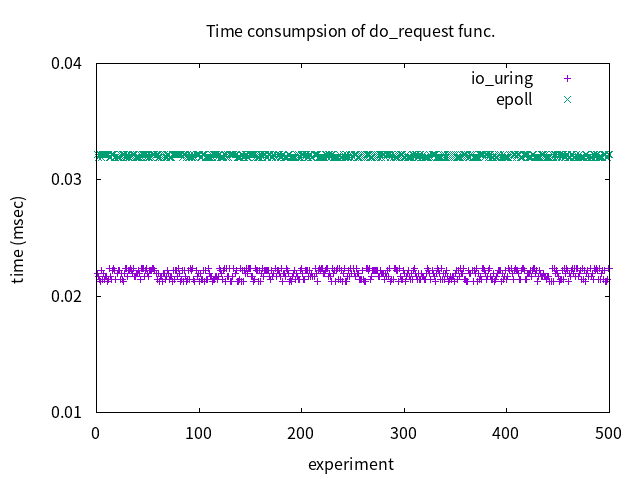
\includegraphics[width=.45\textwidth]{io_uring.png}
  \caption{The comparison of do\_request function}
  \label{Fig:iouring}
\end{wrapfigure}
The healthcare data exchange system would request for "small data" frequently.
Hence, the low latency has the priority over the high throughput in this project.
We often use the system call: "epoll" for asynchronous I/O with many files
descriptors, rather than sequential accessing those file descriptors in this scenario.
Figure \ref*{Fig:iouring} \cite{epoll_vs_iouring} shows that the io\_uring could do
request in fewer time significantly.
\begin{wrapfigure}[10]{R}{.45\textwidth}
  % \centering
  \digraph[scale=.6]{methFlow}{
  Study[margin="0"]
  Combination[margin="0"]
  "Container\noexpand\n Security"[margin="0"]
  "FHIR\noexpand\nSystem"[margin="0"]

  Study -> "Container\noexpand\n Security"-> Combination
  Study -> "FHIR\noexpand\nSystem" -> Combination
  rankdir=LR
  }
  \caption[]{The mapReduce model in this project}
  \label{Fig:model}
\end{wrapfigure}

% ================ Methods ================
\section{Methods}

This project would use the MapReduce model which is shown in Figure \ref*{Fig:model}.

\subsection{Study}
\subsubsection{CVEs and Related Mechanisms}
The Linux kernel is a monolithic kernel, which is over 28 million lines of code now (2020). There
are many mechanisms to solve real-world situations. Studying those CVEs' related mechanism in the
kernel might have more chance to find new vulnerabilities.

This project will study several container vulnerabilities such as CVE-2016-8655
\cite{CVE-2016-8655}, CVE-2016-9962 \cite{CVE-2016-9962}, and CVE-2020-14386 \cite{CVE-2020-14386}.

And we will study some kernel exploit techniques \cite{Kernel_exploitation} because the container shares
the kernel. If we could exploit the kernel in the suffering container, it might have more chance
to influence the other containers or host.

\subsubsection{FHIR and Related Standards}
This project will implement the FHIR \cite{FHIR_home} data exchange system to demonstrate the container
security risk. Hence, we should study the FHIR standard, the JSON format (RFC7159), the XML format
(RFC4825), and RESTful APIs.

\subsubsection{Efficient I/O with `io\_uring`}
This is a new asynchronous I/O API in Linux kernel 5.1 \cite{Efficient_IO_uring}. POSIX has
aio\_read() and aio\_write() to satisfy asynchronous I/O; however, the implementation of those
is most often lackluster and performance is poor. We will study and implement the new asynchronous
I/O API: io\_uring in this project to optimize the performance of the FHIR data exchange system.

\subsection{Container Security}
\subsubsection{Implementation of a Simple Container}
The Linux kernel supplies some system calls to clone a process (also in thread) in their namespace
and group. We could implement a simple container by ourselves so that we can make a list of
vulnerabilities that may happen, which is shown in Figure \ref*{Fig:sc}.

\begin{wrapfigure}[15]{r}{.45\textwidth}
  % \centering
  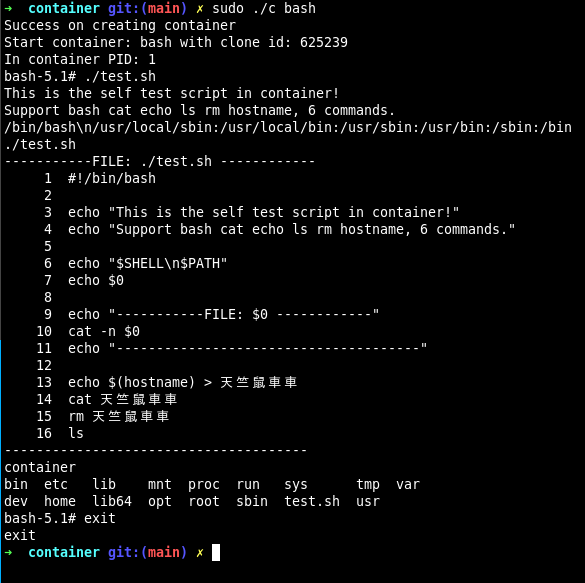
\includegraphics[width=.5\textwidth]{Screenshot from 2021-02-09 19-45-29.png}
  \caption{The implementation of a simple container}
  \label{Fig:sc}
\end{wrapfigure}

\subsubsection{Aimming at Vulnerability and Implementing PoC}
This project would find a vulnerability of privilege escalation in the container and affect
other containers. We would use the fuzzing technique, which is listed from the vulnerabilities
that may happen, to continue researching the security of the Linux kernel in order to detect
other known vulnerabilities of various types, as well as zero-day vulnerabilities \cite{Fuzzing}.

\subsubsection{Implementing Patch and Pull Request}
Being a security researcher, we cannot just only exploit the software, but also give patches to
the maintainer. It will make the container technique more secure.

\subsection{FHIR System}
\subsubsection{Front-End}
This project would design a user-friendly interface. We will make it easy to get data for the
patient and the patient's family. And the exchange of patient's data between different
medical center will be confidential, integral, and available.

The interface would be designed as a website, which makes every user could access on different
platforms.

\subsubsection{Back-End}
This project would use the container technique at the back-end. It would isolate different
services in a different container. We would also design an access controller for variadic
requests, and design a high-performance kernel module to speed up the I/O and caching.

\paragraph{Access Controller}
The access controller would be implemented as a kernel module because a malicious user has
less probability to break the Linux kernel if this module has no bugs.
The access controller would use the whitelisting method to enforce the accessibility policy
\cite{Access_Control_Architecture}.
It would reserve the essential system calls in the container and discard all unused system calls.

\paragraph{High Performance Server}
This project would implement a kernel module for the high performance server, which could hook
the I/O system calls from the web server. The module would replace the normal I/O calls with
io\_uring, which could enhance the concurrency performance to provide low latency and enhance
the throughput.

Moreover, this project would design an efficient algorithm to predict and cache the container's
application data to reduce the latency, while backend server requiring data.

\subsection{System Combination}
The last step is combining the FHIR system and container security. This project would demonstrate
an escalation of normal containers (i.e., Docker) to steal patients' information from the web server.
However, our containers can detect and prevent a malicious user from escaping the container of the
web server.

Furthermore, the performance issue is also the key point in this project. We would provide a
high-performance FHIR system for the real world requirement. Therefore, we would also improve the
I/O performance at the final stage of this project.

% ================ Expected Outcome ================

\section{Expected Outcome}
This project will deploy a secure and high-performance FHIR healthcare data exchange system
in containers. We will demonstrate a container escalation and purpose an efficient mechanism
to protect the patients' privacy. Many companies publish their FHIR system in containers,
that make much medical organization easy to deploy. However, the medical organization might
not have a professional security software engineer to maintain the performance issues and
patients' privacy issues.

Therefore, this project would aim at a secure and high-performance solution for the medical
organization. We hope this could help them face the future cyber challenges.
\paragraph{}
This project has two parts: the FHIR system and container security.
\paragraph{Container Security}
We would implement a vulnerability PoC, patch, and demonstration for container escalation
since the container technique is the trend of these microservices. The healthcare data
exchanging center must use containers for quick deployment and management. Additionally, the
information security issue becomes more and more important these days. To prevent the
cracker from breaking the healthcare data center and keep the patients' information is critical
today. We hope that this research could make the container technique more secure, and provide
the healthcare data exchange system more reliable.

\paragraph{FHIR System}
We would implement the healthcare data exchange system with the FHIR standard. The implementation
would provide a high-performance service for anyone, anywhere, and anytime. The fifth-generation
mobile telecommunications has been launched, and the sixth-generation mobile telecommunications is
coming.  More IoT devices will collect our healthcare data for medical demands, needing a low
latency server to digest the data. We hope that this project could implement a high-performance FHIR
standard system, which makes data exchange effectively.
\paragraph{}
Finally, this project would combine these two parts into a container of a secure and
high-performance FHIR system. It is expected that this project could play the model role of the
healthcare data exchange system in Taiwan.

\printbibliography[heading=bibnumbered]

\section{Academic Advisor}
\begin{itemize}
  \item Give advices of security issues.
  \item Give advices of the front-end of user interface.
  \item Introduce the vision of healthcare data exchanging system.
  \item Organize this research to a complete structure.
  \item Extend the result to a formal paper, and submit it to a conference or a journal.
\end{itemize}

\end{document}
